% ============================================================
%  Sprawozdanie: Badanie dyfrakcji światła (DYFRA)
%  Fotonika – laboratorium, ZUT Szczecin
% ============================================================
\documentclass[a4paper,12pt]{article}

\usepackage[utf8]{inputenc}
\usepackage[T1]{fontenc}
\usepackage[polish]{babel}
\usepackage{geometry}
\geometry{a4paper, top=2.2cm, bottom=2.2cm, left=2.5cm, right=2.5cm}

\usepackage{amsmath,amssymb}
\usepackage{booktabs}
\usepackage{graphicx}
\usepackage{float}
\usepackage{caption}
\usepackage{multirow}
\usepackage{array}
\usepackage{xcolor}
\usepackage{hyperref}
\usepackage{siunitx}
\sisetup{output-decimal-marker={,}, locale=DE}
\usepackage{parskip}
\setlength{\parskip}{4pt}

\title{}
\date{}

\begin{document}

% ============================================================
%  TABELA NAGŁÓWKOWA (punkty 1–3)
% ============================================================
\begin{table}[H]
\centering
\renewcommand{\arraystretch}{1.4}
\begin{tabular}{|p{4.2cm}|p{4.2cm}|p{4.2cm}|}
\hline
\multicolumn{3}{|p{12.9cm}|}{%
  \centering
  \textbf{Zachodniopomorski Uniwersytet Technologiczny w~Szczecinie}
  \newline
  Wydział Elektryczny\quad--\quad Katedra Telekomunikacji i~Fotoniki
  \newline
  \textbf{FOTONIKA -- Laboratorium}
  \newline
  \textbf{Ćwiczenie 03: Badanie dyfrakcji światła (DYFRA)}
} \\
\hline
Prowadzący: Mgr.~Inż.~Eliza Miśkiewicz &
  Kierunek: TI, Studia: S2 & Nr zespołu: 5, Grupa: L1 \\
\hline
\multicolumn{2}{|l|}{Skład zespołu: 1.~Kamil Suchy} &
  Prowadzący: \phantom{X} \\
\hline
\multicolumn{2}{|l|}{Data wykonania ćwiczenia: 13.04.2026\quad Rok: 2025/2026} &
  Ocena: \phantom{XXXXX} \\
\hline
\end{tabular}
\end{table}

% ============================================================
\section*{4.\quad Cel ćwiczenia}
% ============================================================

Celem ćwiczenia jest:
\begin{enumerate}
  \item Wyznaczenie długości fali lasera półprzewodnikowego przy pomocy siatki
        dyfrakcyjnej.
  \item Pomiar szerokości szczeliny na podstawie obrazu dyfrakcyjnego (dyfrakcja
        Fraunhofera) z~uwzględnieniem niepewności systematycznych.
  \item Sprawdzenie słuszności zasady Babineta przez obserwację obrazów dyfrakcyjnych
        szczeliny i~komplementarnego paska o~tej samej szerokości.
\end{enumerate}

% ============================================================
\section*{5.\quad Wstęp teoretyczny}
% ============================================================

\textbf{Dyfrakcja} jest to ugięcie fali na krawędzi przeszkody lub szczeliny.
Dyfrakcja Fraunhofera (pole dalekie) zachodzi, gdy odległość ekranu od przeszkody
$d \gg D = a^2/\lambda$ (odległość Rayleigha), gdzie $a$ jest charakterystycznym
wymiarem przeszkody, a~$\lambda$ -- długością fali.

\textbf{Siatka dyfrakcyjna.} Dla siatki o~stałej $a$ (odległości między szczelinami)
ugięcie wiązki $m$-tego rzędu następuje pod kątem $\alpha_m$ spełniającym warunek:
\begin{equation}
  \sin\alpha_m = \frac{m\lambda}{a}, \label{eq:siatka}
\end{equation}
co pozwala wyznaczyć długość fali:
\begin{equation}
  \lambda = a\cdot\sin\alpha_m.
\end{equation}

\textbf{Dyfrakcja na szczelinie.} Minima dyfrakcji (wygaszenia) jednorodnej szczeliny
o~szerokości $d$ występują dla kątów:
\begin{equation}
  d\cdot\sin\alpha_m = m\lambda \quad\Rightarrow\quad d = \frac{m\lambda}{\sin\alpha_m},
  \label{eq:szczelina}
\end{equation}
gdzie $m = 1,2,3,\ldots$ jest rzędem minimum.

\textbf{Zasada Babineta.} Obrazy dyfrakcyjne komplementarnych przeszkód (np. szczeliny
i~paska o~tej samej szerokości) są identyczne w~obszarze pola dalekiego,
z~wyjątkiem centrum obrazu (prążek zerowy).

\textbf{Kąt ugięcia.} Kąt $\alpha_m$ wyznacza się geometrycznie:
\begin{equation}
  \sin\alpha_m = \frac{x_m}{\sqrt{x_m^2 + L^2}},
\end{equation}
gdzie $L$ -- odległość od elementu dyfrakcyjnego do ekranu, $x_m$ -- odległość
od centrum obrazu do prążka (minimum) rzędu $m$. Dla małych kątów stosuje
się przybliżenie $\sin\alpha \approx \tan\alpha = x/L$.

% ============================================================
\section*{6.\quad Schemat układu pomiarowego}
% ============================================================

\begin{figure}[H]
  \centering
  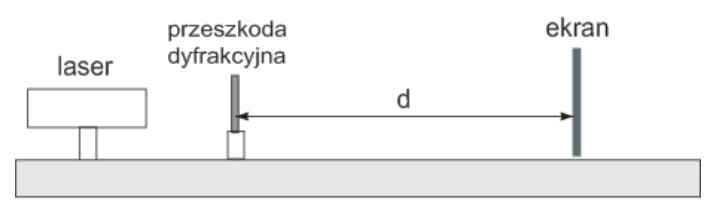
\includegraphics[width=0.82\textwidth]{schemat ukladu pomiarowego.png}
  \caption{Schemat układu pomiarowego do badania dyfrakcji światła.}
  \label{fig:schemat}
\end{figure}

% ============================================================
\section*{7.\quad Spis przyrządów pomiarowych}
% ============================================================

\begin{itemize}
  \item Laser półprzewodnikowy DPSS (zielony), nominalna długość fali
        $\lambda_0 = \SI{532}{nm}$.
  \item Siatka dyfrakcyjna, gęstość linii $N = 530\,\text{l/mm}$,
        stała siatki $a = 1/N = \SI{1{,}887}{\micro m}$,
        niepewność $\Delta a = \SI{0{,}05}{\micro m}$.
  \item Płytka szklana z~7~szczelinami i~7~druckami o~szerokościach
        30, 40, 60, 80, 100, 150, \SI{200}{\micro m}; użyte: szczelina 1
        (\SI{80}{\micro m}), szczelina 2 (\SI{60}{\micro m}).
  \item Miarka milimetrowa (dokładność odczytu $\Delta x = \Delta L = \SI{1}{mm}$).
  \item Ława optyczna.
  \item Ekran.
\end{itemize}

% ============================================================
\section*{8.\quad Przebieg ćwiczenia}
% ============================================================

\begin{enumerate}
  \item \textbf{Wyznaczanie długości fali (część A).} Na drodze wiązki laserowej
        ustawiono siatkę dyfrakcyjną ($N = 530\,\text{l/mm}$). Na ekranie obserwowano
        prążki 1. rzędu dyfrakcji. Zmierzono odległości $L$ (od siatki do ekranu)
        oraz $x$ (od prążka zerowego do prążka 1. rzędu) dla trzech ustawień
        ekranu ($L = 150, 200, 240\,\text{mm}$).

  \item \textbf{Wyznaczanie szerokości szczeliny (część B).} Siatka zastąpiona
        płytką z~szczelinami. Dla \textbf{szczeliny~1} (nominalna
        $d_1^{\text{nom}} = \SI{80}{\micro m}$) zmierzono odległość od centrum
        obrazu do 3.~minimum dyfrakcyjnego ($m = 3$) przy $L = \SI{940}{mm}$.
        Dla \textbf{szczeliny~2} (nominalna $d_2^{\text{nom}} = \SI{60}{\micro m}$)
        zmierzono odległość do 6.~minimum ($m = 6$) przy $L = \SI{965}{mm}$.

  \item \textbf{Sprawdzenie zasady Babineta (część C).} Przy szczelinie
        $d = \SI{80}{\micro m}$ i~komplementarnym drucikiem tej samej szerokości
        porównano położenia minimów dyfrakcyjnych na ekranie dla obu przeszkód.
\end{enumerate}

% ============================================================
\section*{9.\quad Wyniki pomiarów i opracowanie}
% ============================================================

% ─────────────────────────────────────────────────────────────
\subsection*{9.1\quad Tabela~A – Wyznaczanie długości fali lasera}

Stała siatki: $a = \dfrac{1}{530}\,\text{mm} = \SI{1{,}8868}{\micro m}$,
niepewność $\Delta a = \SI{0{,}05}{\micro m}$.
Dokładność miarki: $\Delta x = \Delta L = \SI{1}{mm}$, niepewność standardowa
$u_x = u_L = \Delta/\!\sqrt{3} = \SI{0{,}5774}{mm}$.

\begin{table}[H]
\centering
\caption{Wyniki pomiarów do wyznaczenia długości fali lasera.}
\label{tab:A}
\renewcommand{\arraystretch}{1.3}
\begin{tabular}{
  c
  S[table-format=2.0]
  S[table-format=1.0]
  S[table-format=1.4]
  S[table-format=3.0]
  S[table-format=1.0]
  S[table-format=1.4]
  S[table-format=1.4]
  S[table-format=1.2]
  S[table-format=1.4]
  S[table-format=1.4]
  S[table-format=1.4]
}
\toprule
Lp. &
  {$x$} &
  {$\Delta x$} &
  {$u_x$} &
  {$L$} &
  {$\Delta L$} &
  {$u_L$} &
  {$\sin\alpha$} &
  {$\delta a$} &
  {$\lambda$} &
  {$u(\lambda)$} &
  {$U_\lambda$} \\
 &
  {[mm]} &
  {[mm]} &
  {[mm]} &
  {[mm]} &
  {[mm]} &
  {[mm]} &
  {} &
  {[\%]} &
  {[\textmu m]} &
  {[\textmu m]} &
  {[\textmu m]} \\
\midrule
1 & 42 & 1 & 0,5774 & 150 & 1 & 0,5774 & 0,2800 & 2,65 & 0,5283 & 0,0159 & 0,0318 \\
2 & 56 & 1 & 0,5774 & 200 & 1 & 0,5774 & 0,2800 & 2,65 & 0,5283 & 0,0151 & 0,0302 \\
3 & 67 & 1 & 0,5774 & 240 & 1 & 0,5774 & 0,2792 & 2,65 & 0,5267 & 0,0147 & 0,0295 \\
\bottomrule
\end{tabular}
\end{table}

\noindent\textbf{Obliczenia do Tabeli~A:}

\medskip
\noindent Stała siatki i~jej względna niepewność:
\[
  a = \frac{1}{530}\,\text{mm} = \SI{1{,}8868}{\micro m}, \qquad
  \frac{\Delta a}{a} = \frac{0{,}05}{1{,}8868} = 0{,}02650 \quad (2{,}65\,\%).
\]

\noindent Niepewności standardowe pomiarów odległości ($\Delta x = \Delta L = \SI{1}{mm}$):
\[
  u_x = u_L = \frac{\Delta}{\sqrt{3}} = \frac{1}{\sqrt{3}} = \SI{0{,}5774}{mm}.
\]

\noindent Kąt ugięcia (przybliżenie $\sin\alpha \approx \tan\alpha = x/L$):
\[
  \sin\alpha \approx \frac{x}{L}.
\]

\noindent Długość fali:
\[
  \lambda = a \cdot \sin\alpha \approx a \cdot \frac{x}{L}.
\]

\noindent Lp.~1: $x = 42\,\text{mm}$, $L = 150\,\text{mm}$:
\[
  \sin\alpha = \frac{42}{150} = 0{,}2800, \qquad
  \lambda = 1{,}8868 \times 0{,}2800 = \SI{0{,}5283}{\micro m}.
\]

\noindent Lp.~2: $x = 56\,\text{mm}$, $L = 200\,\text{mm}$:
\[
  \sin\alpha = \frac{56}{200} = 0{,}2800, \qquad
  \lambda = 1{,}8868 \times 0{,}2800 = \SI{0{,}5283}{\micro m}.
\]

\noindent Lp.~3: $x = 67\,\text{mm}$, $L = 240\,\text{mm}$:
\[
  \sin\alpha = \frac{67}{240} = 0{,}27917, \qquad
  \lambda = 1{,}8868 \times 0{,}27917 = \SI{0{,}5267}{\micro m}.
\]

\noindent Niepewność $u(\lambda)$ wyznaczona ze wzoru na propagację niepewności:
\[
  u(\lambda) = \lambda \sqrt{\left(\frac{u_x}{x}\right)^{\!2}
                            + \left(\frac{u_L}{L}\right)^{\!2}
                            + \left(\frac{\Delta a}{a}\right)^{\!2}}.
\]

\noindent Lp.~1:
\[
  u(\lambda) = 0{,}5283 \cdot \sqrt{\left(\frac{0{,}5774}{42}\right)^{\!2}
                                    + \left(\frac{0{,}5774}{150}\right)^{\!2}
                                    + (0{,}02650)^2}
             = 0{,}5283 \cdot \sqrt{1{,}89 \times 10^{-4}
                                    + 1{,}48 \times 10^{-5}
                                    + 7{,}02 \times 10^{-4}}
             = \SI{0{,}0159}{\micro m}.
\]

\noindent Lp.~2:
\[
  u(\lambda) = 0{,}5283 \cdot \sqrt{\left(\frac{0{,}5774}{56}\right)^{\!2}
                                    + \left(\frac{0{,}5774}{200}\right)^{\!2}
                                    + (0{,}02650)^2}
             = 0{,}5283 \cdot \sqrt{1{,}06 \times 10^{-4}
                                    + 8{,}34 \times 10^{-6}
                                    + 7{,}02 \times 10^{-4}}
             = \SI{0{,}0151}{\micro m}.
\]

\noindent Lp.~3:
\[
  u(\lambda) = 0{,}5267 \cdot \sqrt{\left(\frac{0{,}5774}{67}\right)^{\!2}
                                    + \left(\frac{0{,}5774}{240}\right)^{\!2}
                                    + (0{,}02650)^2}
             = 0{,}5267 \cdot \sqrt{7{,}43 \times 10^{-5}
                                    + 5{,}79 \times 10^{-6}
                                    + 7{,}02 \times 10^{-4}}
             = \SI{0{,}0147}{\micro m}.
\]

\noindent Niepewność rozszerzona ($K = 2$): $U_\lambda = K \cdot u(\lambda)$.

\medskip
\noindent Średnia długość fali:
\[
  \bar{\lambda} = \frac{0{,}5283 + 0{,}5283 + 0{,}5267}{3}
                = \SI{0{,}5278}{\micro m} = \SI{527{,}8}{nm}.
\]

\[
  \boxed{\lambda = (0{,}528 \pm 0{,}032)\,\si{\micro m}}
\]

\noindent Wartość nominalna lasera: $\lambda_0 = \SI{532}{nm}$.
Odchylenie względne: $(532 - 527{,}8)/532 \approx 0{,}8\,\%$ -- wynik zgodny.

% ─────────────────────────────────────────────────────────────
\subsection*{9.2\quad Tabela~B – Wyznaczanie szerokości szczeliny}

Do obliczeń przyjęto nominalną długość fali lasera $\lambda = \SI{532}{nm} = \SI{0{,}532}{\micro m}$.

\medskip
\noindent\textbf{Szczelina~1} (nominalna $d_1^{\text{nom}} = \SI{80}{\micro m}$),
3.~minimum dyfrakcyjne ($m = 3$):

\begin{table}[H]
\centering
\caption{Wyniki pomiarów dla szczeliny~1 ($d_1^{\text{nom}} = \SI{80}{\micro m}$, $m = 3$).}
\label{tab:B1}
\renewcommand{\arraystretch}{1.3}
\begin{tabular}{
  S[table-format=2.0]
  S[table-format=1.0]
  S[table-format=1.4]
  S[table-format=3.0]
  S[table-format=1.0]
  S[table-format=1.4]
  S[table-format=1.5]
  S[table-format=1.6]
  S[table-format=2.2]
  S[table-format=1.2]
}
\toprule
{$x$} & {$\Delta x$} & {$u_x$} &
{$L$} & {$\Delta L$} & {$u_L$} &
{$A$} & {$U_A$} &
{$d$} & {$U_d$} \\
{[mm]} & {[mm]} & {[mm]} &
{[mm]} & {[mm]} & {[mm]} &
{} & {} &
{[\textmu m]} & {[\textmu m]} \\
\midrule
20 & 1 & 0,5774 & 940 & 1 & 0,5774 & 0,02127 & 0,00123 & 75,04 & 4,33 \\
\bottomrule
\end{tabular}
\end{table}

\noindent\textbf{Obliczenia – Szczelina~1:}

\[
  A = \sin\alpha_m = \frac{1}{\sqrt{1+(L/x)^2}}
    = \frac{1}{\sqrt{1+(940/20)^2}}
    = \frac{1}{\sqrt{2210}}
    = 0{,}02127.
\]
\[
  d = \frac{m\lambda}{A} = \frac{3 \times 0{,}532}{0{,}02127}
    = \SI{75{,}04}{\micro m}.
\]
\[
  u_d = d\sqrt{\left(\frac{u_x}{x}\right)^{\!2} + \left(\frac{u_L}{L}\right)^{\!2}}
      = 75{,}04 \cdot \sqrt{\left(\frac{0{,}5774}{20}\right)^{\!2}
                            + \left(\frac{0{,}5774}{940}\right)^{\!2}}
      = 75{,}04 \cdot 0{,}02887
      = \SI{2{,}167}{\micro m}.
\]
\[
  U_d = K \cdot u_d = 2 \times 2{,}167 = \SI{4{,}33}{\micro m}.
\]
\[
  u_A = A \cdot \sqrt{\left(\frac{u_x}{x}\right)^{\!2} + \left(\frac{u_L}{L}\right)^{\!2}}
      = 0{,}02127 \times 0{,}02887 = 6{,}14 \times 10^{-4}, \quad
  U_A = 2 \times 6{,}14 \times 10^{-4} = 1{,}23 \times 10^{-3}.
\]

\[
  \boxed{d_1 = (75{,}0 \pm 4{,}3)\,\si{\micro m}}
\]
Wartość nominalna: $d_1^{\text{nom}} = \SI{80}{\micro m}$.
Odchylenie względne: $(80 - 75{,}0)/80 = 6{,}3\,\%$.

\bigskip
\noindent\textbf{Szczelina~2} (nominalna $d_2^{\text{nom}} = \SI{60}{\micro m}$),
6.~minimum dyfrakcyjne ($m = 6$):

\begin{table}[H]
\centering
\caption{Wyniki pomiarów dla szczeliny~2 ($d_2^{\text{nom}} = \SI{60}{\micro m}$, $m = 6$).}
\label{tab:B2}
\renewcommand{\arraystretch}{1.3}
\begin{tabular}{
  S[table-format=2.0]
  S[table-format=1.0]
  S[table-format=1.4]
  S[table-format=3.0]
  S[table-format=1.0]
  S[table-format=1.4]
  S[table-format=1.5]
  S[table-format=1.6]
  S[table-format=2.2]
  S[table-format=1.2]
}
\toprule
{$x$} & {$\Delta x$} & {$u_x$} &
{$L$} & {$\Delta L$} & {$u_L$} &
{$A$} & {$U_A$} &
{$d$} & {$U_d$} \\
{[mm]} & {[mm]} & {[mm]} &
{[mm]} & {[mm]} & {[mm]} &
{} & {} &
{[\textmu m]} & {[\textmu m]} \\
\midrule
50 & 1 & 0,5774 & 965 & 1 & 0,5774 & 0,05170 & 0,00120 & 61,74 & 1,43 \\
\bottomrule
\end{tabular}
\end{table}

\noindent\textbf{Obliczenia – Szczelina~2:}

\[
  A = \frac{1}{\sqrt{1+(965/50)^2}}
    = \frac{1}{\sqrt{373{,}89}}
    = 0{,}05170.
\]
\[
  d = \frac{m\lambda}{A} = \frac{6 \times 0{,}532}{0{,}05170}
    = \SI{61{,}74}{\micro m}.
\]
\[
  u_d = 61{,}74 \cdot \sqrt{\left(\frac{0{,}5774}{50}\right)^{\!2}
                            + \left(\frac{0{,}5774}{965}\right)^{\!2}}
      = 61{,}74 \cdot \sqrt{(0{,}01155)^2 + (5{,}98 \times 10^{-4})^2}
      = 61{,}74 \cdot 0{,}01156
      = \SI{0{,}714}{\micro m}.
\]
\[
  U_d = 2 \times 0{,}714 = \SI{1{,}43}{\micro m}.
\]
\[
  u_A = 0{,}05170 \times 0{,}01156 = 5{,}98 \times 10^{-4}, \quad
  U_A = 2 \times 5{,}98 \times 10^{-4} = 1{,}20 \times 10^{-3}.
\]

\[
  \boxed{d_2 = (61{,}7 \pm 1{,}4)\,\si{\micro m}}
\]
Wartość nominalna: $d_2^{\text{nom}} = \SI{60}{\micro m}$.
Odchylenie względne: $(61{,}7 - 60)/60 = 2{,}8\,\%$.

% ─────────────────────────────────────────────────────────────
\subsection*{9.3\quad Tabela~3 – Sprawdzenie zasady Babineta}

Szerokość szczeliny i~komplementarnego paska: $d = \SI{80}{\micro m}$.
Odległość ekranu od przeszkody: $L = \SI{940}{mm}$.

\begin{table}[H]
\centering
\caption{Porównanie położeń minimów dyfrakcyjnych dla szczeliny i~paska
         (zasada Babineta).}
\label{tab:babinet}
\renewcommand{\arraystretch}{1.3}
\begin{tabular}{cccc}
\toprule
Szerokość szczeliny / paska &
  Rząd minimum &
  Szczelina $x_m$ &
  Pasek $x_m$ \\
\midrule
\multirow{3}{*}{$d = \SI{80}{\micro m}$}
  & $m_1 = 3$ & \SI{19}{mm} & \SI{19}{mm} \\
  & $m_2 = 4$ & \SI{25}{mm} & \SI{25}{mm} \\
  & $m_3 = 5$ & \SI{30}{mm} & \SI{30}{mm} \\
\bottomrule
\end{tabular}
\end{table}

\noindent Dla porównania -- teoretyczne położenia minimów ze wzoru $x_m = m\lambda L/d$:
\begin{align*}
  x_3 &= \frac{3 \times 532 \times 10^{-9} \times 0{,}940}{80 \times 10^{-6}}
       = \SI{18{,}8}{mm} \approx \SI{19}{mm}, \\
  x_4 &= \frac{4 \times 532 \times 10^{-9} \times 0{,}940}{80 \times 10^{-6}}
       = \SI{25{,}0}{mm} \approx \SI{25}{mm}, \\
  x_5 &= \frac{5 \times 532 \times 10^{-9} \times 0{,}940}{80 \times 10^{-6}}
       = \SI{31{,}3}{mm} \approx \SI{30}{mm}.
\end{align*}

\noindent Zmierzone położenia są zgodne (w granicy niepewności pomiaru
$\Delta x \approx \SI{1}{mm}$) z~wartościami teoretycznymi. Minima dla
szczeliny i~paska pokrywają się we wszystkich zbadanych rzędach,
co potwierdza zasadę Babineta.

% ============================================================
\section*{10.\quad Wnioski}
% ============================================================

\begin{enumerate}
  \item \textbf{Długość fali lasera} wyznaczona metodą siatki dyfrakcyjnej:
        $\lambda = (0{,}528 \pm 0{,}032)\,\si{\micro m}$.
        Wartość jest zgodna z~nominalną długością fali lasera DPSS
        $\lambda_0 = \SI{532}{nm}$; odchylenie względne wynosi zaledwie
        ok.~$0{,}8\,\%$. Dominującym źródłem niepewności jest niepewność
        stałej siatki~$\Delta a/a \approx 2{,}65\,\%$.

  \item \textbf{Szerokość szczeliny~1} wyznaczona z~3.~minimum dyfrakcyjnego:
        $d_1 = (75{,}0 \pm 4{,}3)\,\si{\micro m}$, wartość nominalna
        $d_1^{\text{nom}} = \SI{80}{\micro m}$.
        Odchylenie wynosi ok.~$6\,\%$, co mieści się w~granicach dopuszczalnych
        tolerancji produkcyjnych płytki z~szczelinami. Stosunkowo duża niepewność
        wynika z~małej odległości $x = \SI{20}{mm}$, co powoduje dużą względną
        niepewność $u_x/x \approx 2{,}9\,\%$.

  \item \textbf{Szerokość szczeliny~2} wyznaczona z~6.~minimum dyfrakcyjnego:
        $d_2 = (61{,}7 \pm 1{,}4)\,\si{\micro m}$, wartość nominalna
        $d_2^{\text{nom}} = \SI{60}{\micro m}$.
        Wynik jest bardzo dobry -- odchylenie od wartości nominalnej wynosi
        zaledwie $2{,}8\,\%$. Pomiar wyższego rzędu ($m = 6$) przy dłuższej
        odległości $L$ poprawia dokładność, ponieważ zwiększa $x$, a~co za tym
        idzie zmniejsza względną niepewność $u_x/x$.

  \item \textbf{Zasada Babineta} została potwierdzona doświadczalnie: minima
        dyfrakcyjne dla szczeliny ($d = \SI{80}{\micro m}$) i~komplementarnego
        paska tej samej szerokości pokrywają się we wszystkich trzech zbadanych
        rzędach ($m = 3, 4, 5$) z~dokładnością $\pm\SI{1}{mm}$, co jest zgodne
        z~teorią dyfrakcji Fraunhofera.

  \item Porównanie niepewności obu metod wyznaczania szerokości szczeliny
        pokazuje, że większa odległość ekranu $L$ i~wyższy rząd minimum
        ($m$) zapewniają mniejszą względną niepewność pomiaru~$d$.
        Należy jednak dbać, by warunek pola dalekiego $L \gg a^2/\lambda$
        był zachowany.
\end{enumerate}

\end{document}
